% Required for hand-in: None
% Required for solution: PICTURES/error_cancellation.eps, MATLAB/cancellation.m

\renewcommand{\chpt}{ch_matvec}

\begin{problem}[Avoiding cancellation \coreproblem] \label{prb:cancellation}
  In \lref{sec:cancel} we saw that the so-called \emph{cancellation phenomenon} is
  a major cause of numerical instability, \emph{cf.} \lref{par:cancel}. Cancellation
  is the massive amplification of \emph{relative errors} when subtracting two
  real numbers of about the same value. 

  Fortunately, expressions vulnerable to cancellation can often be recast in
  a mathematically equivalent form that is no longer affected by cancellation,
  see \lref{par:cancelrem}. There we studied several examples, and this problem
  gives some more.

%  The following problems are taken from \cite[Chapter 2.5, pag. 35ff.]{Ascher}. For
%  additional exercises on the same subject, refer to the source.
 
 \begin{subproblem}[1]
   We consider the function
   \begin{gather}
     \label{eq:cancel:1}
     f_1(x_0,h) := \sin(x_0 + h) - \sin(x_0)\;.
   \end{gather}
   It  can the transformed into another form, $f_2(x_0,h)$, using the trigonometric identity
   \[
   \sin(\varphi) - \sin(\psi) = 2 \cos \left(\frac{\varphi + \psi}{2} \right) \sin \left(\frac{\varphi - \psi}{2} \right).
   \]
   Thus, $f_1$ and $f_2$ give the same values, in exact arithmetic, for any given argument values $x_0$ and $h$.
  
  \begin{enumerate}
   \item Derive $f_2(x_0,h)$, which does no longer involve the difference of
     return values of trigonometric functions.
   \item Suggest a formula that avoids cancellation errors for computing the
     approximation ($f(x_0 + h) - f(x_0)) / h$) of the derivative of
     $f(x) := \sin(x)$ at $x = x_0$. Write a \Matlab~ program that implements your
     formula and computes an approximation of $f'(1.2)$, for
     $h = 1 \cdot 10^{-20}, 1 \cdot 10^{-19},\cdots,1$.
     
     \begin{hint}
       For background information refer to \lref{ex:canceldiffq}.
     \end{hint}

   \item Plot the error (in doubly logarithmic scale using \matlab's
     \texttt{loglog} plotting function) of the derivative computed with the
     suggested formula and with the naive implementation using $f_1$.
   \item Explain the observed behaviour of the error.
  \end{enumerate}
  
  \begin{solution}
   Check the \Matlab{} implementation in \cref{mc:cancellation} and the plot in \cref{fig:error_cancellation}. We can clearly observe that the computation using $f_1$ leads to a big error as $h \rightarrow 0$. This is due to the cancellation error given by the subtraction of two number of approximately same magnitude. The second implementation using $f_2$ is very stable and does not display round-off errors.
   
   \lstinputlisting[language=matlab,caption={\Matlab{} script for \ref{prb:cancellation}},label={mc:cancellation}]{\problems/\chpt/MATLAB/cancellation.m}

    \begin{figure}[htb]
    \centering
    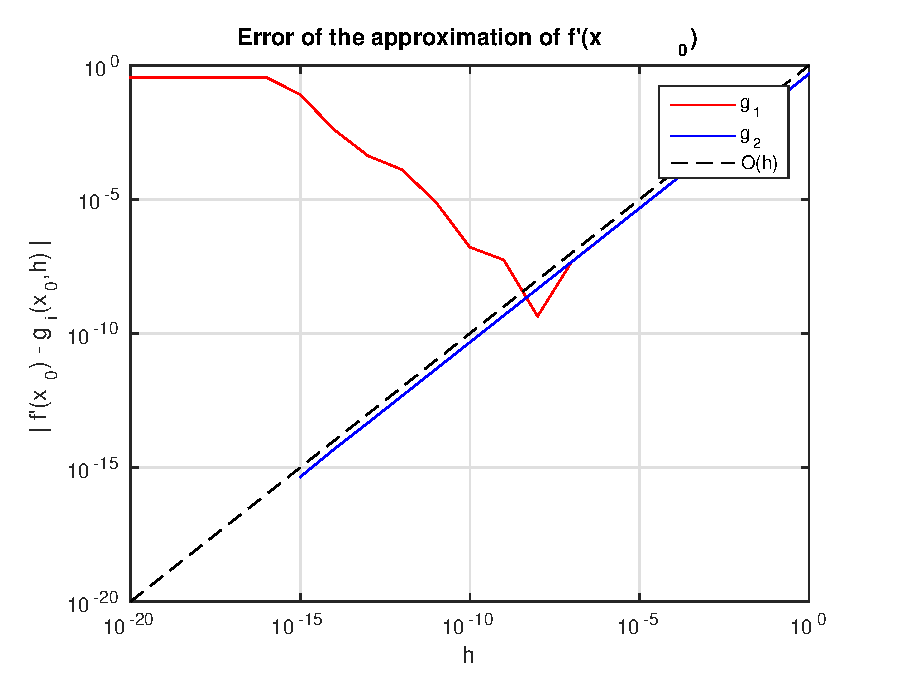
\includegraphics[width=0.8\textwidth]{\problems/\chpt/PICTURES/error_cancellation.eps}
    \caption{Timings for \ref{prb:cancellation}} \label{fig:error_cancellation}
    \end{figure}
  \end{solution}


 \end{subproblem}
 
 \begin{subproblem}[2]
   Using a trick applied in \lref{ex:canctrig} show that
  \begin{gather*}
    \ln(x - \sqrt{x^2 - 1}) = - \ln( x + \sqrt{x^2 - 1})\;.
  \end{gather*}
  Which of the two formulas is more suitable for numerical computation? Explain
  why, and provide a numerical example in which the difference in accuracy is
  evident.
   
  \begin{solution}
 We immediately derive $\ln(x - \sqrt{x^2 - 1}) + \ln(x + \sqrt{x^2 - 1}) = \log(x^2 - (x^2 - 1)) = 0$. As $x \rightarrow \infty$ the left $\log$ consists of subtraction of two numbers of equal magnitude, whilst the right $\log$ consists on the addition of two numbers of approximately the same magnitude. Therefore, in the first case there may be cancellation for large values of $x$, making it worse for numerical computation. Try, in \Matlab, with $x = 10^8$.
  \end{solution}

 \end{subproblem}

 \begin{subproblem}[2]
  For the following expressions, state the numerical difficulties that may occur, and rewrite the formulas in a way that is more suitable for numerical computation.
  \begin{enumerate}
   \item $\sqrt{x + \frac{1}{x}} - \sqrt{x - \frac{1}{x}}$, where $x \gg 1$.
   \item $\sqrt{\frac{1}{a^2} + \frac{1}{b^2}}$, where $a \approx 0, b \approx 1$.
  \end{enumerate}
  
  \begin{solution}
  \begin{enumerate}
   \item Inside the square roots we have the addition (rest. subtraction) of a small number to a big number. The difference of the square roots incur in cancellation, since they have the same, large magnitude. $A := x + \frac{1}{x}, B := x - \frac{1}{x}$ then $(A-B)(A+B)/(A+B) = \frac{2/x}{\sqrt{x + \frac{1}{x}} + \sqrt{x - \frac{1}{x}}} = \frac{2}{\sqrt{x} (\sqrt{x^2 + 1} + \sqrt{x^2 - 1})}$
   \item $\frac{1}{a^2}$ becomes very large as $a$ approaches $0$, whilst $\frac{1}{b^2} \rightarrow 1$ as $b \rightarrow 1$. Therefore, the relative size of $\frac{1}{a^2}$ and $\frac{1}{b^2}$ becomes so big, that, in computer arithmetic, $\frac{1}{a^2} + \frac{1}{b^2} = \frac{1}{a^2}$. On the other hand
   $\frac{1}{a}\sqrt{1+(\frac{a}{b})^{2}}$ avoids this problem by performing a division between two numbers with very different magnitude, instead of a summation.
  \end{enumerate}
  \end{solution}
 \end{subproblem}
\end{problem}
 